\documentclass[x11names]{article}
\usepackage{tikz}
\usepackage{pgfplots}
\usepackage{xcolor}
\usepackage{svg}
\usepackage{amsmath}
\usepackage{array}
\usepackage[skins]{tcolorbox}
\usepackage[version=4]{mhchem}
\usepackage[a4paper, total={6in, 10in}]{geometry}
%\usepackage{fouriernc}
\usepackage{xymtex}
\usepackage{textcomp}
\usepackage{eurosym}
\usepackage{mathrsfs}
\usepackage{float}
\usepackage{pst-all}
\usepackage{pst-3dplot}
\usepackage{leftindex}
\usepackage{verbatim}
\usepackage{import}
\usepackage{xifthen}
\usepackage{pdfpages}
\usepackage{transparent}
\usepackage{import}
\usepackage{pdfpages}
\usepackage{transparent}
\usepackage{amssymb}
%\usepackage{graphicx}


\definecolor{myblue}{RGB}{224, 245, 255} 
\definecolor{myred}{RGB}{234, 222, 255}
\definecolor{myorange}{RGB}{255, 102, 0}

% box
\newtcolorbox{es}[2][]{%
	enhanced,colback=white,colframe=black,coltitle=black,
	sharp corners,boxrule=0.4pt,
	fonttitle=\itshape,
	attach boxed title to top left={yshift=-0.5\baselineskip-0.4pt,xshift=2mm},
	boxed title style={tile,size=minimal,left=0.5mm,right=0.5mm,
		colback=white,before upper=\strut},
	title=#2,#1
}

% definizioni
\newtcolorbox{blues}[2][]{%
	enhanced,colback=myblue,colframe=black,coltitle=black,
	sharp corners,boxrule=0.4pt,
	attach boxed title to top left={yshift=-0.5\baselineskip-0.4pt,xshift=2mm},
	boxed title style={tile,size=minimal,left=0.5mm,right=0.5mm,
		colback=myblue,before upper=\strut},
	title=#2,#1
}

% teoremi
\newtcolorbox{redes}[2][]{%
	enhanced,colback=myred,colframe=black,coltitle=black,
	sharp corners,boxrule=0.4pt,
	fonttitle=\itshape,
	attach boxed title to top left={yshift=-0.5\baselineskip-0.4pt,xshift=2mm},
	boxed title style={tile,size=minimal,left=0.5mm,right=0.5mm,
		colback=myred,before upper=\strut},
	title=#2,#1
}


%% regole
\renewcommand*\contentsname{Indice}
\setcounter{tocdepth}{4}
\setcounter{secnumdepth}{2}
\pgfplotsset{compat=1.15}


\usetikzlibrary{arrows}


\title{Letteratura italiana}
\author{Federico Cesari}
\date{}



\begin{document}
	
\begin{titlepage}
	\begin{center}
		\vspace*{1cm}
		
		\textbf{\LARGE Relazione di laboratorio - Pendolo semplice}
		
		\vspace{0.3cm}
		\large \textit{Misura del periodo di un pendolo semplice} \\
		
		\vspace{0.5cm}
		\Large Federico Cesari \\
		
		\small 1096759 
		\vspace{0.2cm}
		
		\small Gruppo 5
		
		
		\vspace{3cm}
		\begin{center}
			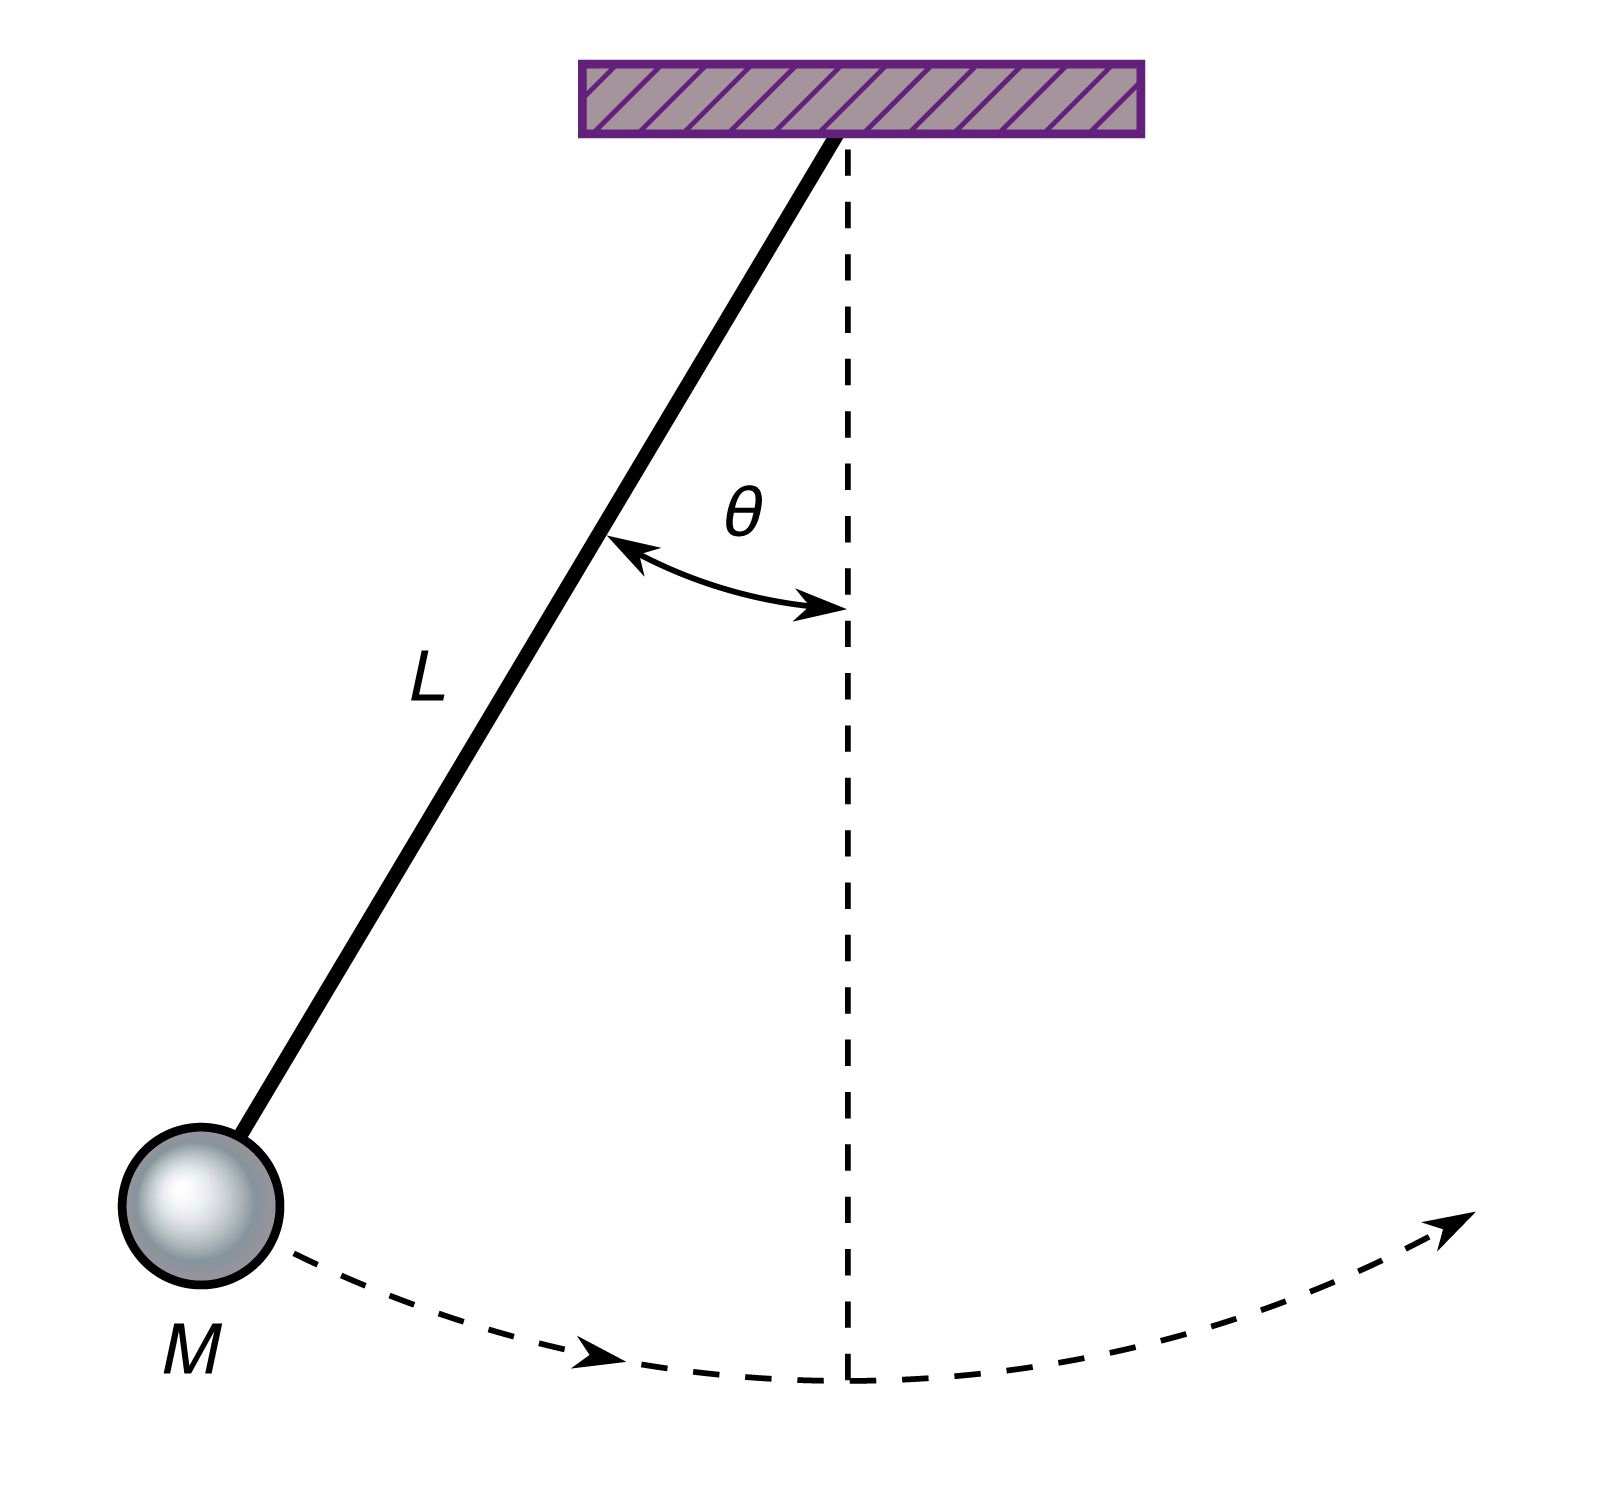
\includegraphics[scale=0.1]{IMG_0200.jpeg}	
		\end{center}
		
		
		
		\vfill
		
		
		
		corso A\\
		Università degli studi di Torino, Torino\\
		4 aprile 2024\\
		
		
	\end{center}
\end{titlepage}
\tableofcontents
\newpage


\begin{center}
\fboxsep11pt
\colorbox{myblue}{\begin{minipage}{5.75in}
	\begin{blues}{Definizione: }
	\end{blues}
\end{minipage}}       
\end{center}

\begin{center}
\fboxsep11pt
\colorbox{myred}{\begin{minipage}{5.75in}
	\begin{redes}{}
	\subsubsection{Teorema  }
	\end{redes}
\end{minipage}}        
\end{center}



% DOCUMENT %



\section{Serie numeriche}
Sia \(a_{n} \subset \mathbb{C}\) successione di numeri complessi, chiamiamo \textbf{serie numerica} la sommatoria 
\[ 
\sum_{n=0}^{\infty} a_{n} = a_{1} + \dots + a_{n} + \dots
\]
Chiamiamo invece \textbf{ridotta ennesima} della serie la quantità
\[ 
S_{N} = \sum_{n=0}^{N} a_{n} = a_{1} + \dots + a_{N} \qquad N \in \mathbb{N}
\]
Abbiamo costruito la \textbf{successione delle ridotte} \(S_{N}\) con \(N\in\mathbb{N}\).

	\subsection{Successioni di numeri complessi}
	\begin{center}
		\fboxsep11pt
		\colorbox{myblue}{\begin{minipage}{5.75in}
				\begin{blues}{Definizione: Serie convergente divergente e indeterminata}
					Se il limite 
					\[ 
					\lim_{N\to\infty}S_{N} = S \in \mathbb{C}
					\]
					diciamo che la serie 
					\[ 
					\sum_{n=0}^{\infty} a_{n} = S
					\]
					converge ad \(S\) e chiamiamo \(S\) somma della serie. \\
					
					Nel caso in cui \(S_{N}\) sia divergente o indeterminata la serie è divergente o indeterminata.
				\end{blues}
		\end{minipage}}       
	\end{center}
	
	
	\subsection{Carattere di una serie}
	Si osserva che preso \(n_{0} \in \mathbb{N}\) e considerando la serie
	\[ 
	\sum_{n=n_{0}}^{\infty} a_{n} \quad \text{questa ha lo stesso carattere di }\quad \sum_{n=0}^{\infty} a_{n}
	\]
	Chiaramente la somma sarà diversa, il carattere tuttavia non cambia.
	\begin{center}
		\fboxsep11pt
		\colorbox{myred}{\begin{minipage}{5.75in}
				\begin{redes}{}
					\subsubsection{Teorema: Condizione necessaria di convergenza}
					Sia \(a_{n} \subset \mathbb{C}\). Condizione necessaria affinché la serie
					\[ 
					sum_{n=0}^{\infty} a_{n}
					\]
					converga è che 
					\[ 
					\lim_{n\to \infty} a_{n} = 0
					\]
				\end{redes}
		\end{minipage}}        
	\end{center}
	
	\begin{center}
		\fboxsep11pt
		\colorbox{myred}{\begin{minipage}{5.75in}
				\begin{redes}{}
					\subsubsection{Teorema: "Linearità delle serie"}
					Prendiamo due serie di numeri complessi convergenti rispettivamente ad \(A\) e a \(B\):
					\[ 
					sum_{n=0}^{\infty} a_{n} = A \qquad\qquad sum_{n=0}^{\infty} b_{n} = B
					\]
					allora
					\[ 
					i) \qquad \forall \lambda \in \mathbb{C} \quad  \sum_{n=0}^{\infty} \lambda a_{n} = \lambda \sum_{n=0}^{\infty}  a_{n}= \lambda A
					\]
					\[ 
					ii) \qquad \sum_{n=0}^{\infty}  (a_{n} + b_{n} )= \sum_{n=0}^{\infty} a_{n} + \sum_{n=0}^{\infty} b_{n} = A + B
					\]
				\end{redes}
		\end{minipage}}        
	\end{center}
	
	\subsection{Serie geometrica, serie telescopiche e armoniche}
	Fissato \(q \in \mathbb{C}\) si dice \textbf{serie geometrica} di ragione \(q\) la serie
	\[ 
	\sum_{n=0}^{\infty} q^n = \frac{1-q^{N+1}}{1-q}
	\]
	il carattere è determinato da \(q\):
	\[ 
	\begin{array}{lc}
		|q| < 1 & \text{la serie converge} \\
		|q| > 1 \text{ o } q = 1 & \text{la serie diverge} \\
		|q| = 1 \text{ e } q \neq 1 & \text{la serie è indeterminata} \\
	\end{array}
	\] \\
	
	\noindent
	Chiamiamo \textbf{serie telescopiche} le seguenti le serie di forma
	\[ 
	a_{0} + \sum_{n=1}^{\infty} (a_{n} - a_{n-1}) \qquad a_{n} \subset \mathbb{C}
	\]
	\begin{es}{alcuni esempi di serie telescopiche}
		\begin{minipage}{0.5\textwidth}
			\[ 
			i) \qquad \sum_{n=1}^{\infty} \frac{1}{n(n+1)} = 1
			\]
		\end{minipage}
		\begin{minipage}{0.5\textwidth}
			\[ 
			ii) \qquad \sum_{n=1}^{\infty} \log\left(1 + \frac{1}{n}\right) = +\infty
			\]
		\end{minipage}
	\end{es}	
	
	\subsection{Serie a termini non negativie a segni alterni}
	
	\[ 
	\text{Termini non negativi} \qquad \sum_{n=0}^{\infty} a_{n}, \qquad a_{n} \geq 0, \qquad \forall n \in \mathbb{N}
	\]
	\[ 
	\text{Segni alterni} \quad \qquad \sum_{n=0}^{\infty} (-1)^nb_{n}, \qquad b_{n} > 0, \qquad \forall n \in \mathbb{N}
	\]
	\begin{center}
		\fboxsep11pt
		\colorbox{myred}{\begin{minipage}{5.75in}
				\begin{redes}{}
					\subsubsection{Teorema: Le serie a termini non negativi o convergono o divergono}
					Sia \(a_{n}\) una serie a termini non negativi, questa può o convergere o divergere, non può essere indeterminata.
				\end{redes}
		\end{minipage}}        
	\end{center}
	\begin{es}{dimostrazione}
		Prendo \(\{S_{N}\}_{N\in\mathbb{N}}\) \textbf{monotona crescente}:
		\[ 
		S_{N+1} = S_{N} + a_{N+1} \geq S_{N}
		\]
		Se il limite converge a \(S\) limite superiore 
		\[ 
		\lim_{N\to\infty} S_{N} = S \in [0,+\infty)  \qquad S = \text{sup }_{S\in\mathbb{N}} S_{N}
		\]
		\[ 
		\Longrightarrow \text{ La serie converge}
		\]
		Se \(\{S_{N}\}_{N\in\mathbb{N}}\) non è superiormente limitata si ha 
		\[ 
		\lim_{N\to\infty} S_{N} = +\infty
		\]
		\[ 
		\Longrightarrow \text{ La serie diverge}
		\]

	\end{es}
	
	\begin{center}
		\fboxsep11pt
		\colorbox{myblue}{\begin{minipage}{5.75in}
				\begin{blues}{Definizione: Convergenza assoluta}
					Sata una serie di numeri complessi \(\sum_{n=0}^{\infty} a_{n} \in \mathbb{C}\) si dice che la serie è \textbf{assolutamente convergente} se è convergente la serie
					\[ 
					\sum_{n=0}^{\infty} |a_{n}|
					\]
				\end{blues}
		\end{minipage}}       
	\end{center}
	\begin{center}
		\fboxsep11pt
		\colorbox{myred}{\begin{minipage}{5.75in}
				\begin{redes}{}
					\subsubsection{Teorema: Convergenza assoluta implica convergenza semplice}
					Sia \(\sum_{n=0}^{\infty} a_{n} \subset \mathbb{C}\). Supponiamo che la serie sia assolutamente convergente, allora la serie è anche semplicemente convergente. Inoltre vale
					\[ 
					\left|\sum_{n=0}^{\infty} a_{n}\right| \leq \sum_{n=0}^{\infty} |a_{n}|
					\]
				\end{redes}
		\end{minipage}}        
	\end{center}
	\subsection{Criteri applicabili alle serie}
	\begin{itemize}
		\item{Criterio del confronto}
		\item{Criterio del confronto asintotico}
		\item{\textbf{Criterio della radice:}} \\
		 Sia \(\sum a_{n}\) serie a termini positivi. Supponiamo che esista
		\[ 
		\lim_{n\to \infty} \sqrt[n]{a_{n}} = \lim a^{1/n}_{n} = l \in [0,+\infty]
		\]
		allora 
		\[ 
		\begin{array}{ll}
			l<1 & \text{la serie converge} \\
			l>1 & \text{la serie diverge} \\
			l=1 & \text{caso dubbio}
		\end{array}
		\]
		\item{\textbf{Criterio del rapporto:}} \\
		 Sia \(\sum a_{n}\) serie a termini positivi. Supponiamo \(a_{n} > 0 \forall n\) e che esista
		\[ 
		\lim_{n\to \infty} \frac{a_{n+1}}{a_{n}} =  l \in [0,+\infty]
		\]
		allora 
		\[ 
		\begin{array}{ll}
			l<1 & \text{la serie converge} \\
			l>1 & \text{la serie diverge} \\
			l=1 & \text{caso dubbio}
		\end{array}
		\]
		\item{Criterio dell'integrale di Mc. Laurin}
		\item{\textbf{Criterio di Leibniz:}} \\
		Sia data la serie \(\sum_{n=0}^{\infty}(-1)^n b_{n}\) con \(b_{n} > 0 \forall n\). Supponiamo
		\[ 
		\begin{array}{l}
			1) \qquad b_{n+1} \leq b_{n} \quad \forall n \qquad \text{(la serie è decrescente)} \\
			2) \qquad \lim_{n\to\infty} b_{n} = 0
		\end{array}
		\]
		Allora la serie converge a 
		\[ 
		S = \sum_{n=0}^{\infty}(-1)^nb_{n}
		\]
		e \(|S - S_{N}| \leq b_{N+1} \quad \forall N \in \mathbb{N}\).
	\end{itemize}
		
		
	\begin{es}{}
		\subsection{Procedimento per la risoluzione degli esercizi}
		\begin{enumerate}
			\item Verificare la condizione necessaria di convergenza
			\item Se è a \textbf{valori non negativi}: 
				\begin{enumerate}
					\item Tramite confronto e confronto asintotico verificare se questa converge o diverge.
				\end{enumerate}
			\item Se è a \textbf{segni alterni}:
				\begin{enumerate}
					\item Ne studio il modulo;
					\item Tramite confronto e confronto asintotico verificare se questa converge o diverge assolutamente;
					\item Se diverge uso il \textbf{criterio di Leibniz};
					\item Verifico che sia strettamente decrescente;
					\item Se lo è la serie è semplicemente convergente.
				\end{enumerate}
		\end{enumerate}
	\end{es}
	
\newpage
\section{Topologia di \(\mathbb{R}^n\)}
Questa sezione contiene solo definizioni, non sto a distinguerle con il riquadro colorato.

\subsubsection*{Intorno}
Si dice \textbf{intorno sferico} di centro \(x_{0} \in \mathbb{R}^n\) e raggio \(r>0\) l'insieme
\[ 
B(x_{0},r) = \{x \in \mathbb{R}^n \quad |\quad d(x,x_{0}) = |x-x_{0}| < r\}
\]
La distanza dalle due dimensioni in poi chiaramente è espressa come
\[ 
d(x,x_{0}) = \sqrt{(x-x_{0})^2 + (y-y_{0})^2 + \dots }
\]


\subsubsection*{Punto di accumulazione}
Sia \(A \subseteq \mathbb{R}^n\) e \(x_{0} \in \mathbb{R}^n\). Si dice \textbf{punto di accumulazione} per \(A\) se
\[ 
\forall r > 0 \qquad \left(B(x_{0},r) \textbackslash \{x_{0}\} \right) \cap A \neq \varnothing
\]
\textit{In sostanza è un punto di accumulazione se ogni suo intorno contiene punti di \(A\) diversi da se stesso}
\subsubsection*{Insieme limitato}
\(A \subseteq \mathbb{R}^n\) si dice limitato se
\[ 
\exists M > 0 \quad | \quad \|x\| \leq M, \quad \forall x \in A
\]
\[ 
A \subseteq \overline{B(O,M)} \quad \text{con} \quad B(O,M) = \{x \in \mathbb{R} \quad | \quad \|x\|\leq M \}
\]
\subsubsection*{Insieme aperto}
\(A\subseteq \mathbb{R}^n\) si dice aperto se 
\[ 
\forall x \in A \quad \exists r > 0 \quad | \quad B(x_{o},r) \subset A
\]
\begin{itemize}
	\item	\(\mathbb{R}^n\) è un insieme aperto;
	\item   L'intersezione di qualunque famigia di un chiuso è un aperto,
	\item   L'unione di un numero finito di chiusi è un aperto.
\end{itemize}

\subsubsection*{Insieme chiuso}
\(C\subseteq \mathbb{R}^n\) si dice \textbf{chiuso} se il suo complementare \(\mathbb{R}^n \backslash C\) è un aperto.

\begin{itemize}
	\item	Sono chiusi gli insiemi \(\mathbb{R}^n\) e \(\varnothing\);
	\item  l'intersezione di qualunque famigia di un chiuso è un chiuso;
	\item   l'unione di un numero finito di chiusi è un chiuso.
\end{itemize}


\subsubsection*{Insieme compatto}
Un sottoinsieme \(K\subset \mathbb{R}^n\) è detto \textbf{compatto} se è chiuso e limitato.

\subsubsection*{Putni interni, esterni e di frontiera}
\[ 
\text{Interno:} \qquad \exists r > 0 \quad | \quad B(x_{0}, r) \subset A
\]
\[ 
\text{Interno:} \qquad \exists r > 0 \quad | \quad B(x_{0}, r) \cap A = \varnothing
\]
Se \(x_{0}\) non è né interno né esterno è un putno di frontiera.

\begin{itemize}
	\item	\(Int(A)\) è un aperto ed è il più grande aperto contenuto in \(A\);
	\item   \(Int(A) \cap Fr(A)\) è un chiuso ed è il più piccolo chiuso contenente \(A\) e viene denotato con \(\bar{A}\);
	\item   \(Fr(A)\) è un chiuso;
	\item \(A\) è chiuso \(\Longleftrightarrow\) \(A = Int(A)\);
\end{itemize}

% F.ni SCALARI 

\newpage
\section{Calcolo differenziale per funzioni scalari}
	
	% DERIVATE PRIME e DIFFERENZIABILITA
	
	\subsection{Derivate parziali}
	
		\subsubsection{Derivate cartesiane}
		\subsubsection{Derivate direzionali}

		\begin{center}
		\fboxsep11pt
		\colorbox{myblue}{\begin{minipage}{5.75in}
			\begin{blues}{Definizione: Gradiente di un campo scalare}
			\end{blues}
		\end{minipage}}       
		\end{center}

	\subsection{Differenziabilità}
		%differenziale campo scalare
		\begin{center}
		\fboxsep11pt
		\colorbox{myblue}{\begin{minipage}{5.75in}
			\begin{blues}{Definizione: Differenziabilità}
			\end{blues}
		\end{minipage}}       
		\end{center}

		\begin{center}
		\fboxsep11pt
		\colorbox{myred}{\begin{minipage}{5.75in}
			\begin{redes}{}
			\subsubsection{Teorema: differenziabilità implica esistenza della derivata direzionale}
			\end{redes}
		\end{minipage}}        
		\end{center}

		\begin{center}
		\fboxsep11pt
		\colorbox{myred}{\begin{minipage}{5.75in}
			\begin{redes}{}
			\subsubsection{Teorema: differenziabilità implica continità}
			\end{redes}
		\end{minipage}}        
		\end{center}

		\begin{center}
		\fboxsep11pt
		\colorbox{myred}{\begin{minipage}{5.75in}
			\begin{redes}{}
			\subsubsection{Teorema: condizione sufficiente di differenziabilità}
			\end{redes}
		\end{minipage}}        
		\end{center}
	
	\subsection{Derivata lungo una curva}
	\subsection{Ortogonalità del gradiente alle curve di livello in 2d}
	\subsection{Ortogonalità del gradiente alle curve di livello in 3d}


	% DERIVATE SECONDE

	\subsection{Derivate seconde}

	\begin{center}
	\fboxsep11pt
	\colorbox{myred}{\begin{minipage}{5.75in}
		\begin{redes}{}
		\subsubsection{Teorema di Schwartz}
		\end{redes}
	\end{minipage}}        
	\end{center}

		\subsubsection{Matrice Hessiana}



% F.ni VETTORIALI

\newpage
\section{Calcolo differenziale per funzioni vettoriali}
	\subsection{Curve parametriche}
	
	\subsection{Derivate parziali}
		\subsubsection{Derivate cartesiane}
		\subsubsection{Derivate direzionali}
		\begin{center}
		\fboxsep11pt
		\colorbox{myblue}{\begin{minipage}{5.75in}
			\begin{blues}{Definizione: derivata direzionale}
				\[
				F:A \subseteq \mathbb{R}^n \to \mathbb{R}^m, \qquad \mathbf{\bar{x}} \in \text{Int}(A), \qquad 					      \mathbf{v} \in \mathbb{R}^n, \quad \mathbf{v} \neq 0
				\]
				Si dice \textbf{derivata direzionale} di $F$ lungo $\mathbf{v}$ in  $\mathbf{\bar{x}}$ il limite, se esiste finito,
				\begin{equation}
					\frac{\partial F}{\partial \mathbf{v}}(\mathbf{\bar{x}}) = \lim_{t\to0} \frac{F( \mathbf{\bar{x}} + t \mathbf{v}) - F( \mathbf{\bar{x}} )}{t}
				\end{equation}
				Sia
				\[ 
				F(x) = \left(F_{1}(x),\dots,F_{m}(x)\right),\qquad F_{j}:A\subseteq \mathbb{R}^n\to\mathbb{R}
				\]
				allora per il \textit{Teorema del limite globale}
				\[ 
				\frac{\partial F}{\partial \mathbf{v}}(\mathbf{\bar{x}}) \quad \text{esiste} \quad \Longleftrightarrow \quad \text{esistono} \quad \frac{\partial F_{j}}{\partial 		\mathbf{v}}(\mathbf{\bar{x}}) \quad \forall j = 1,\dots,m
				\]
			\end{blues}
			\end{minipage}}       
		\end{center}

	\subsection{Differenziabilità}
	\begin{center}
	\fboxsep11pt
%	\colorbox{myblue}{\begin{minipage}{5.75in}
%		\begin{blues}{Definizione: Differenziabilità e Matrice Jacobiana}
%			 Sia \(\boldsymbol{\bar{x}} \in Int(A)\). DIciamo che \(F\) è differenziabile in \(\boldsymbol{\bar{x}}\) se esiste una applicazione lineare \(T:\mathbb{R}^n\to \mathbb{R}^m\) tale che
%			 \[ 
%			 F(\boldsymbol{\bar{x}} + \boldsymbol{h}) - F(\boldsymbol{\bar{x}}) = T(\boldsymbol{h}) + o(\|\boldsymbol{h}\|), \quad \boldsymbol{h} \to \boldsymbol{0}
%			 \]
%			 \(T:\mathbb{R}^n\to \mathbb{R}^m\) è lineare quidi esiste una matrice \(B\) \(m\times n\) tale che
%			 \[ 
%			 T(\boldsymbol{h}) = B\boldsymbol{h}
%			 \] 
%			 Usando il teorema del limite globale, \(F(\boldsymbol{x}) = (F_{1}(\boldsymbol{x}),\dots,F_{m}(\boldsymbol{x}))\) è differenziabile in \(\boldsymbol{\bar{x}}\) se e solo se \(F_{j}(\boldsymbol{x})\) è differenziabile in \(\boldsymbol{\bar{x}}\) \(\forall j = 1,\dots,m\). \\
%			 
%			 Definiamo la \textbf{matrice jacobiana} di \(F\) in \(\boldsymbol{\bar{x}}\)
%			 \[ 
%			 JF(\boldsymbol{\bar{x}}) = 
%			 \left(\begin{array}{cccc}
%			 	\partial_{x_{1}}F_{1}(\boldsymbol{\bar{x}}) & \partial_{x_{2}}F_{1}(\boldsymbol{\bar{x}}) & \cdots & \partial_{x_{n}}F_{1}(\boldsymbol{\bar{x}}) &  \\
%			 	\partial_{x_{1}}F_{2}(\boldsymbol{\bar{x}}) & \partial_{x_{2}}F_{2}(\boldsymbol{\bar{x}}) & \cdots & \partial_{x_{n}}F_{2}(\boldsymbol{\bar{x}}) &  \\
%			 	\cdots & \ddots & \ddots & \vdots \\
%			 	\partial_{x_{1}}F_{m}(\boldsymbol{\bar{x}}) & \partial_{x_{2}}F_{m}(\boldsymbol{\bar{x}}) & \cdots & \partial_{x_{n}}F_{m}(\boldsymbol{\bar{x}}) &  
%			 \end{array}\right) 
%			 \begin{array}{c}
%			 \textcolor{red}{\nabla F_{1}(\boldsymbol{\bar{x}})} \\
%			 \textcolor{red}{\nabla F_{2}(\boldsymbol{\bar{x}})} \\
%			 \textcolor{red}{\vdots} \\
%			 \textcolor{red}{\nabla F_{m}(\boldsymbol{\bar{x}})} \\
%			 \end{array}
%			 \]
%		\end{blues}
%	\end{minipage}}      
	\end{center}
	%differenziale campo vettoriale 

	\subsection{Composizione di campi vettoirali}
	\begin{center}
	\fboxsep11pt
	\colorbox{myred}{\begin{minipage}{5.75in}
		\begin{redes}{}
		\subsubsection{Chain rule}
		\end{redes}
	\end{minipage}}        
	\end{center}

	\subsection{Cambio di coordinate}

	\subsection{Operatore di Laplace}

	\subsection{Teorema di inversione locale}
	\begin{center}
	\fboxsep11pt
	\colorbox{myred}{\begin{minipage}{5.75in}
		\begin{redes}{}
		\subsubsection{TIL}
		Sia \(A \subseteq \mathbb{R}^n\) aperto e \(T:A\subseteq \mathbb{R}^n \to \mathbb{R}^n\) con \(T\in \mathcal{C}^1(A)\). 
		
		Sia \(x_{0} \in A\) e \(y_{0} = T(x_{0})\).
		
		Supponiamo \(\text{det}\left[JT(x_{0})\right] \neq 0\). Allora:
		\begin{enumerate}
			\item Esiste un intorno aperto \(U\) di \(x_{0}\) tale che \(T(U)\) sia un intorno aperto di \(y_{0}\) e la funzione
			\[ 
			T: U \to T(U)
			\]
			sia biettiva.
			\item La funzione inversa locale 
			\[ 
			T^{-1}: T(U) \to U
			\]
			è di classe \(\mathcal{C}^1\) su \(T(U)\) e \(JT^{-1}(y_{0}) = \left[JT(x_{0})\right]^{-1}\)
		\end{enumerate}
		\end{redes}
	\end{minipage}}        
	\end{center}
	\subsection{Teoremi della funzione implicita}
	\begin{center}
	\fboxsep11pt
	\colorbox{myred}{\begin{minipage}{5.75in}
		\begin{redes}{}
		\subsubsection{TFI in 2 dimensioni}
		Sia \(A \subseteq \mathbb{R}^2\) aperto e \(f: A\to \mathbb{R}\) campo scalare di classe \(\mathcal{C^1}\) su \(A\): \(f\in \mathcal{C}^1(A)\). \\
		
		Definiamo un punto \(P_{0}\) appartenente all'insieme di livello \(\Sigma_c = \{(x,y) \in A : f(x,y) = c\}\):
		\[
		P_{0} = (x_{0},y_{0}) \quad | \quad f(x_{0},y_{0}) = c
		\]
		
		Valgono le seguenti affermazioni:
		\begin{enumerate}
			\item Se \(\frac{\partial f}{\partial y}(P_{0}) \neq 0\) allora esiste un rettangolo 
			\[ 
			I\times J = (x_{0} - a, x_{0} + a) \times (y_{0} - b, y_{0} + b) \qquad a,b > 0
			\]
			tale che l'insieme intersezione del rettangolo con l'insieme di livello
			\[ 
			\{f=c\} \cap (I\times J) = \{(x,y) \in I \times J : f(x,y) = c\}
			\]
			è il grafico di una funzione 
			\[ 
			y = \varphi(x)
			\]
		\end{enumerate}
		\end{redes}
	\end{minipage}}        
	\end{center}
	\begin{center}
	\fboxsep11pt
	\colorbox{myred}{\begin{minipage}{5.75in}
		\begin{redes}{}
		\subsubsection{TFI in 3 dimensioni}
		\end{redes}
	\end{minipage}}        
	\end{center}



\end{document}



 
